% 度量空间
% 度量空间|欧几里得空间|距离函数

\pentry{集合\upref{Set}}

\begin{definition}{度量空间}
一个集合中任意两个元素 $u, v$ 间若定义了满足以下条件的\textbf{距离函数(distance function)} $d(u, v)$ (函数值为实数), 那它就是一个\textbf{度量空间}. 集合中的每个元素就叫空间中的一个\textbf{点}.
\begin{itemize}
\item 正定性:$d(u, v) \geq 0$,且$d(u, v)=0$当且仅当$u=v$
\item 对称性:$d(u, v) = d(v, u)$
\item 三角不等式:$d(u, v) \leqslant d(u, w) + d(w, v)$
\end{itemize}
\end{definition}
%修改批注:将原先的四个条件整合成三个条件,并冠以数学界习惯的名称,方便学生记忆.

\begin{exercise}{欧几里得空间}
$N$ 维欧几里得空间 $\mathbb R^N$ 中若定义距离函数为
\begin{equation}
d(x, y) = \sqrt{\sum_{i=1}^N (x_i - y_i)^2}
\end{equation}
那么它是一个度量空间.
\end{exercise}

度量空间是除拓扑空间\upref{Topol}外最广义的空间.
\begin{figure}[ht]
\centering
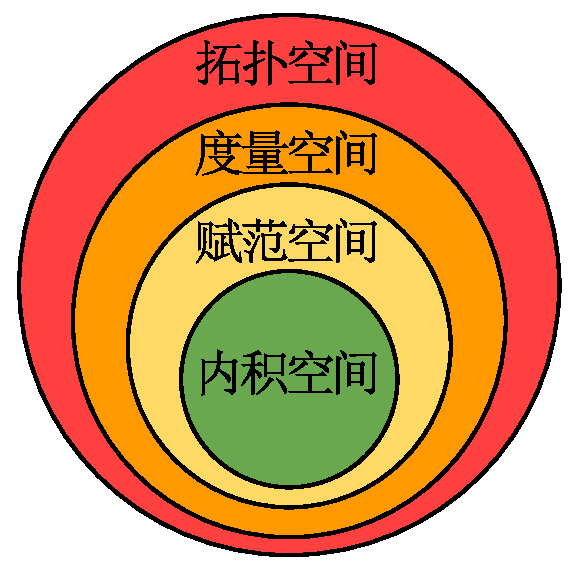
\includegraphics[width=5cm]{./figures/Metric_2.pdf}
\caption{用维恩图表示几种不同空间之间的关系, 从内到外分别是内积空间\upref{InerPd}, 赋范空间\upref{NormV}, 度量空间, 拓扑空间\upref{Topol}(修改自维基百科)} \label{Metric_fig2}
\end{figure}

\subsection{开集和闭集}

\begin{definition}{邻域}
给定一个半径 $r > 0$, 度量空间 $X$ 中的一点 $x$ 周围所有满足 $d(x, y) < r$ 的点 $y$(包括 $x$ 自己)就是 $x$ 的一个\textbf{邻域(neighborhood)} $N_r$. 如果将邻域去掉 $x$ 本身, 就叫做\textbf{去心邻域(deleted/punctured neighbourhood)}.
\end{definition}

\begin{definition}{极限点}
给定度量空间 $X$ 中的一点 $x$, 如果对任意的 $r > 0$, $x$ 的去心邻域都不为空, 那么 $x$ 就是一个极限点. 如果一个点不是极限点, 他就是\textbf{离散点}.
\end{definition}

\begin{corollary}{}
度量空间 $X$ 中的点 $x$ 是极限点的充分必要条件是, $x$ 的任意去心邻域都有无穷多个点.
\end{corollary}

例如, 度量空间 $\mathbb R$ 中, 任意一点都是极限点, 有理数集合构成的度量空间中任意一点也是极限点(证明显然).

\begin{definition}{序列的极限}
给定度量空间 $X$ 中的无穷个点组成的序列 $x_1, x_2, \dots$ 以及一点 $x \in X$, 若对任意给定的 $\epsilon > 0$, 总存在 $N$ 使得当 $n > N$ 时就有 $d(x_n, x) < \epsilon$, 那么 $x$ 就是该序列的极限.
\end{definition}
注意度量空间中序列的极限未必是极限点, 例如整数集 $\mathbb Z$ 中的序列 $1, 2, 3, 3, 3, \dots$ 的极限是 $3$, 但 $\mathbb Z$ 中任意一点都不是极限点.

% \begin{definition}{集合的极限点}
%(错!)若 $A$ 是度量空间 $X$ 的一个子集, 且 $X$ 的一个极限点 $x$ 的某个去心邻域是 $A$ 的子集, 那么 $x$ 就是子集 $A$ 的一个极限点, 无论 $x$ 是否属于 $A$.
% \end{definition}
例如有理数(作为 $\mathbb R$ 的一个子集)的极限点却不一定是有理数, 例如 $\sqrt{2}$ 的任意邻域中都有无穷个有理数, 但 $\sqrt{2}$ 却是无理数.

我们可以使用距离函数直接定义开集和闭集.
\begin{definition}{度量空间的开集}
给定度量空间 $X$ 的一个子集 $A$, 若对于任意 $x \in A$ 都存在 $r > 0$ 使得邻域 $N_r$ 属于 $A$, 那么 $A$ 就是一个\textbf{开集(open set)}.
\end{definition}

\begin{definition}{闭集}
若度量空间 $X$ 的子集 $A$ 关于 $X$ 的补集都是\textbf{闭集(closed set)}.
\end{definition}

\begin{theorem}{}
度量空间 $X$ 的子集 $A$ 是闭集的充分必要条件是: $A$ 的所有极限点都属于 $A$.
\end{theorem}
